% ==============================================================================
% best_equipo_01.tex: Best Model Deep Dive
% Taller 2 - Predicting Poverty | MECA 4107 | Equipo 1: Aragón, Cadena, Flórez
% Compilar desde 04_Slides con: pdflatex best_equipo_01.tex
% ==============================================================================
\documentclass[aspectratio=169, 10pt]{beamer}
% ==============================================================================
% estilo.tex: formato común de los dos decks (best y compare)
% Taller 2 - Predicting Poverty | MECA 4107 | Equipo 1: Aragón, Cadena, Flórez
% Se compila con pdflatex. Las figuras y tablas salen de 01_Scripts/04_Results
% y 01_Scripts/02_EDA (carpeta 03_Output): ningún número se escribe a mano
% salvo los que también imprimen esos scripts.
% ==============================================================================
\usetheme[progressbar=frametitle, numbering=fraction, block=fill, sectionpage=none]{metropolis}
\usepackage[spanish, es-noshorthands]{babel}
\usepackage[utf8]{inputenc}
\usepackage[T1]{fontenc}
\usepackage[sfdefault, scaled=.92]{FiraSans}
\usepackage{booktabs, threeparttable, makecell, multirow, array, colortbl, xcolor}
\usepackage{tikz}
\usetikzlibrary{positioning, arrows.meta, shapes.geometric, fit, calc}
\graphicspath{{../03_Output/Figures/}}

% Colores (los mismos de las figuras: paleta Okabe-Ito)
\definecolor{azul}{HTML}{0072B2}
\definecolor{naranja}{HTML}{D55E00}
\definecolor{verde}{HTML}{009E73}
\definecolor{rosa}{HTML}{CC79A7}
\definecolor{gris}{HTML}{4D4D4D}
\definecolor{fondo}{HTML}{F4F6F8}
\definecolor{oscuro}{HTML}{1F2A3A}

\setbeamercolor{frametitle}{bg=oscuro, fg=white}
\setbeamercolor{progress bar}{fg=naranja, bg=oscuro!30}
\setbeamercolor{title separator}{fg=naranja}
\setbeamercolor{alerted text}{fg=naranja}
\setbeamercolor{block title}{bg=oscuro!12, fg=oscuro}
\setbeamercolor{block body}{bg=fondo}
\setbeamercolor{normal text}{fg=gris}
\setbeamerfont{frametitle}{size=\large}
\setbeamerfont{footnote}{size=\tiny}

% Tablas de kableExtra: tamaño compacto
\newcommand{\tabla}[2][\footnotesize]{{#1\renewcommand{\arraystretch}{1.15}\input{../03_Output/Tables/#2.tex}}}
% Tabla escalada a un ancho dado: \tablar{ancho}{archivo}
\newcommand{\tablar}[2]{\resizebox{#1}{!}{\input{../03_Output/Tables/#2.tex}}}
% Mensaje principal de la diapositiva (una línea, arriba)
\newcommand{\mensaje}[1]{{\color{oscuro}\bfseries #1}\par\vspace{0.4em}}
% Fuente pequeña al pie
\newcommand{\fuente}[1]{\par\vfill{\tiny\color{gris!80} #1}}
% Cifra grande
\newcommand{\cifra}[2]{\begin{tabular}[t]{@{}c@{}}{\color{naranja}\fontsize{24}{26}\selectfont\bfseries #1}\\[0.1em]\scriptsize #2\end{tabular}}

\title{Predecir la pobreza en Colombia}
\author{Equipo 1: Aragón, Cadena y Flórez}
\institute{MECA 4107 Big Data y Machine Learning para Economía Aplicada --- Universidad de los Andes}
\date{Problem Set 2 \quad\textbullet\quad Octubre de 2026}

\subtitle{Best Model Deep Dive}

\begin{document}

\maketitle

% ------------------------------------------------------------------------------
% Diapositiva obligatoria: el mejor modelo (igual en los dos decks)
\begin{frame}{El mejor modelo en una diapositiva}
\mensaje{Clasificamos con un índice de ingreso construido desde las personas}
\begin{columns}[T]
\begin{column}{0.6\textwidth}
\resizebox{\linewidth}{!}{% Diagrama del mejor modelo (se usa en los dos decks)
\begin{tikzpicture}[
  font=\scriptsize, >={Stealth[length=2mm]},
  caja/.style={draw=#1, fill=#1!10, rounded corners=3pt, align=center, minimum height=8mm, inner sep=3pt, line width=0.7pt},
  caja/.default=azul, flecha/.style={->, line width=0.7pt, color=gris}]
  % Personas
  \node[caja=naranja, text width=24mm] (per) {\textbf{541 mil personas}\\variables propias\\+ de su hogar};
  \node[caja=naranja, text width=27mm, right=8mm of per, yshift=9mm] (m17) {LightGBM: ingreso total};
  \node[caja=naranja, text width=27mm, right=8mm of per] (m20) {LightGBM: + columnas\\crudas y pesos};
  \node[caja=naranja, text width=27mm, right=8mm of per, yshift=-9mm] (m22) {5 LightGBM: uno por\\componente del ingreso};
  \node[caja=naranja, text width=22mm, right=7mm of m20] (suma) {Suma por hogar\\y promedio: $\hat y$};
  \node[caja=naranja, text width=28mm, right=7mm of suma] (z) {$z = \hat y - g$\\$g$: brecha exacta del DANE\\$\sigma$: error esperado};
  \node[caja=naranja, text width=20mm, below=6mm of z] (logit) {Logit en\\$z,\ z/\sigma,\ \log\sigma$};
  % Hogar
  \node[caja=azul, text width=24mm, below=17mm of per] (hog) {\textbf{165 mil hogares}\\85 variables};
  \node[caja=azul, text width=27mm, right=8mm of hog] (xgb) {XGBoost de\\clasificación};
  % Ensamble
  \node[caja=rosa, text width=34mm, below=6mm of logit] (ens) {$P = 0.3\,P_{\text{XGB}} + 0.7\,P_{\text{ingreso}}$\\pobre si $P \geq 0.40$};
  \draw[flecha] (per.east) -- ++(3mm,0) |- (m17.west);
  \draw[flecha] (per.east) -- (m20.west);
  \draw[flecha] (per.east) -- ++(3mm,0) |- (m22.west);
  \draw[flecha] (m17.east) -- ++(3mm,0) |- (suma.west);
  \draw[flecha] (m20.east) -- (suma.west);
  \draw[flecha] (m22.east) -- ++(3mm,0) |- (suma.west);
  \draw[flecha] (suma) -- (z);
  \draw[flecha] (z) -- (logit);
  \draw[flecha] (logit) -- (ens);
  \draw[flecha] (hog) -- (xgb);
  \draw[flecha] (xgb.east) -- (xgb.east -| ens.west);
\end{tikzpicture}
}
\par\vspace{0.5em}
{\scriptsize\textbf{Especificación (boosting):} $P = 0.3\,P_{\text{XGBoost}} + 0.7\,P_{\text{ingreso}}$. El XGBoost clasifica con 85 variables del hogar. $P_{\text{ingreso}}$: tres LightGBM predicen el ingreso de cada persona; se suma por hogar, se promedian y se compara con la brecha del hogar; un logit lo convierte en probabilidad según qué tan incierta es la predicción ($\sigma$). Pobre si $P \geq 0.40$.\par}
\end{column}
\begin{column}{0.38\textwidth}
\centering
\cifra{0.77}{Kaggle público}\hspace{0.6em}\cifra{0.77}{Kaggle privado}\hspace{0.6em}\cifra{0.776}{F1 CV}
\par\vspace{0.6em}\raggedright
{\footnotesize
\begin{enumerate}\setlength\itemsep{0.25em}
\item \alert{Predecir el ingreso de cada persona} vale más que cambiar de algoritmo.
\item El desbalance se maneja con el \alert{umbral}, no rebalanceando.
\item Sin el módulo de ingresos, una encuesta corta cae a \alert{F1 0.69}.
\end{enumerate}}
\par\vspace{0.3em}
{\tiny Cuatro envíos empatan en 0.77 en el público (Kaggle muestra 2 decimales); entre ellos, el CV difiere en menos de 0.001, menos que su error estándar. Presentamos el que el equipo seleccionó.\par}
\end{column}
\end{columns}
\end{frame}


% ------------------------------------------------------------------------------
\section{Datos}

\begin{frame}{La pobreza es una regla sobre el ingreso, y 1 de cada 5 hogares es pobre}
\vspace{-0.4em}
\begin{columns}[c]
\begin{column}{0.58\textwidth}
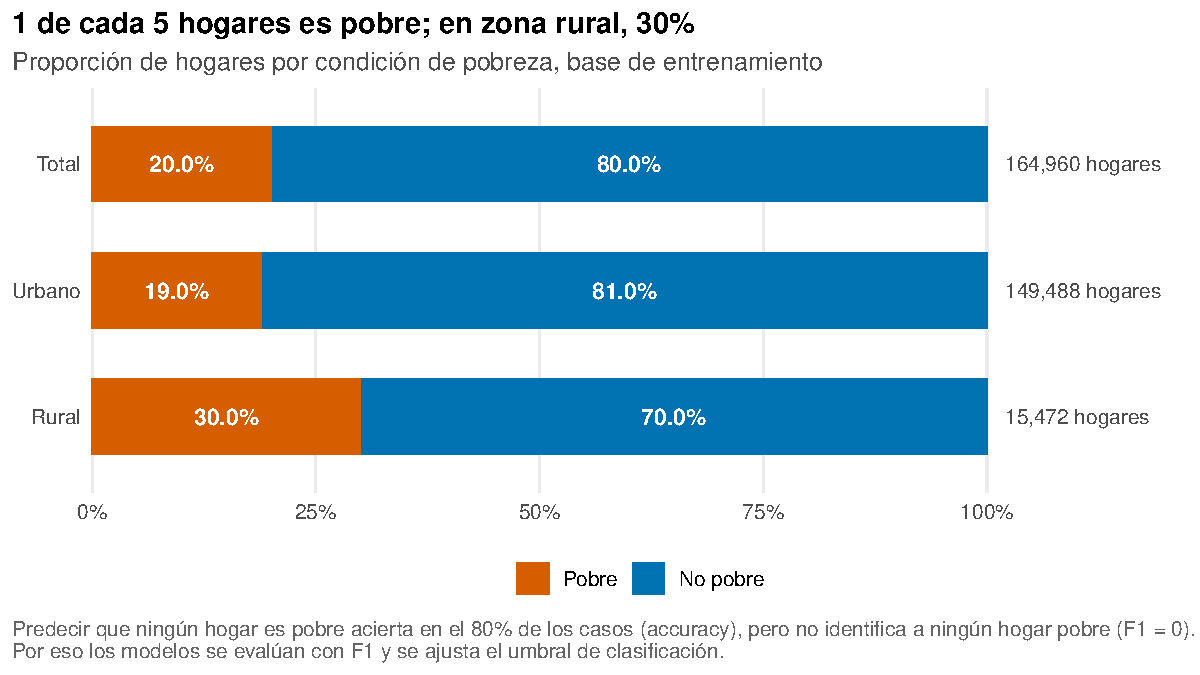
\includegraphics[width=\linewidth]{fig_desbalance.pdf}
\end{column}
\begin{column}{0.4\textwidth}
\begin{block}{Regla oficial del DANE, reescrita}
\centering
$\text{Pobre} = 1 \iff S < G$
\par\vspace{0.3em}\raggedright
{\footnotesize $S = \sum_{j \in UG} \text{Ingtot}_j$: ingreso de las personas\\
$G = L_p \times N_{ug} - R$: brecha ($R$: arriendo imputado)\\
Reproduce el \alert{99.99 \%} de la pobreza de train.}
\end{block}
\end{column}
\end{columns}
\vspace{0.5em}
\begin{columns}[T]
\begin{column}{0.32\textwidth}\footnotesize
\textbf{$G$ se conoce en test} (línea, personas y arriendo): solo hay que predecir $S$.
\end{column}
\begin{column}{0.32\textwidth}\footnotesize
\textbf{$S$ vive en las personas}: el ingreso es la suma de lo que gana cada miembro.
\end{column}
\begin{column}{0.32\textwidth}\footnotesize
\textbf{Desbalance:} 20 \% pobres. Con F1, predecir ``nadie es pobre'' da 0.
\end{column}
\end{columns}
\end{frame}

\begin{frame}{Lo que predice la pobreza: trabajo formal, dependencia y vivienda}
\mensaje{Con empleo formal la pobreza baja a 2--11 \%; con muchos menores y pocos ocupados llega al 93 \%}
\begin{columns}[T]
\begin{column}{0.5\textwidth}
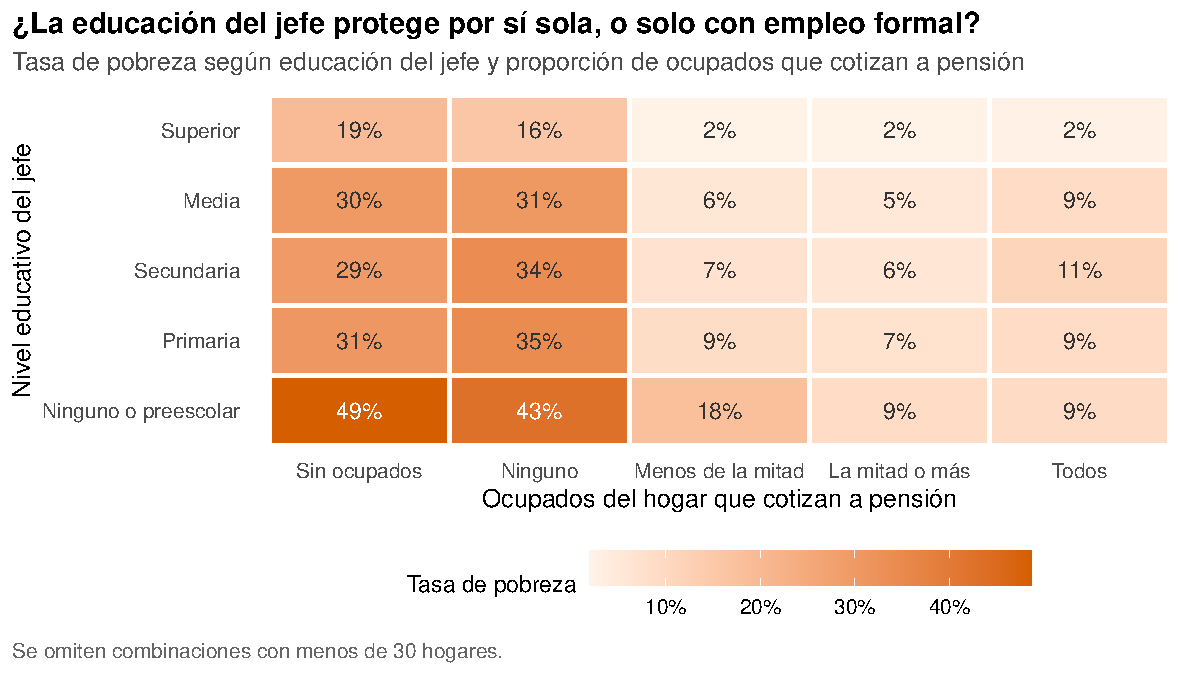
\includegraphics[width=\linewidth]{fig_educ_formalidad.pdf}
\end{column}
\begin{column}{0.5\textwidth}
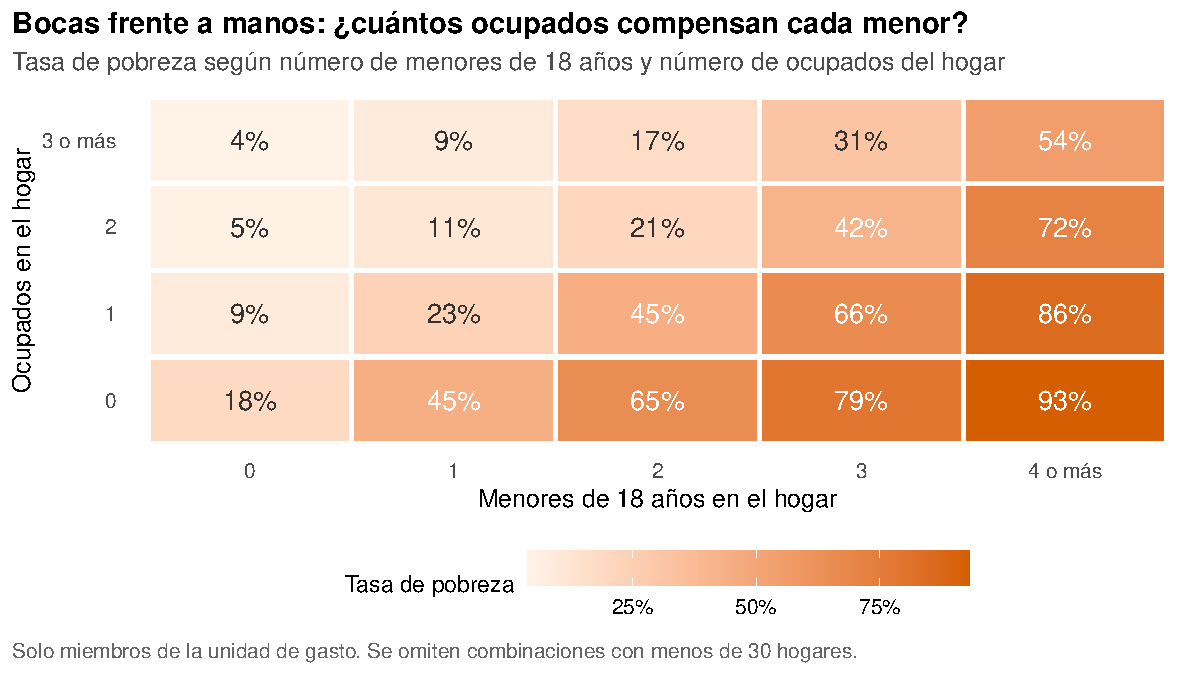
\includegraphics[width=\linewidth]{fig_dependencia.pdf}
\end{column}
\end{columns}
\vspace{0.3em}
{\small Razonamiento económico: el ingreso del hogar $\approx$ ocupados $\times$ calidad del empleo, repartido entre sus miembros. La vivienda (arriendo por persona) resume el ingreso permanente.}
\end{frame}

\begin{frame}{El ingreso tiene cinco fuentes con procesos muy distintos}
\begin{columns}[c]
\begin{column}{0.5\textwidth}
\tablar{\linewidth}{tab_componentes}
\vspace{0.6em}

{\small Los componentes suman exactamente \texttt{Ingtot} en el 100 \% de las personas de train.}
\end{column}
\begin{column}{0.48\textwidth}
\begin{block}{Por qué modelar a las personas}
\small
\begin{itemize}
\item El salario depende de la \alert{posición ocupacional}, la cotización y el oficio de cada miembro.
\item Las \alert{pensiones} son el 12 \% del ingreso pero las recibe el 5 \% de las personas: un monto grande y casi fijo.
\item Un modelo a nivel hogar solo ve promedios; uno por persona ve \alert{quién} genera el ingreso.
\end{itemize}
\end{block}
\end{column}
\end{columns}
\end{frame}

% ------------------------------------------------------------------------------
\section{El mejor modelo}

\begin{frame}{Cómo llegamos aquí: 21 envíos, cuatro etapas}
\begin{columns}[c]
\begin{column}{0.72\textwidth}
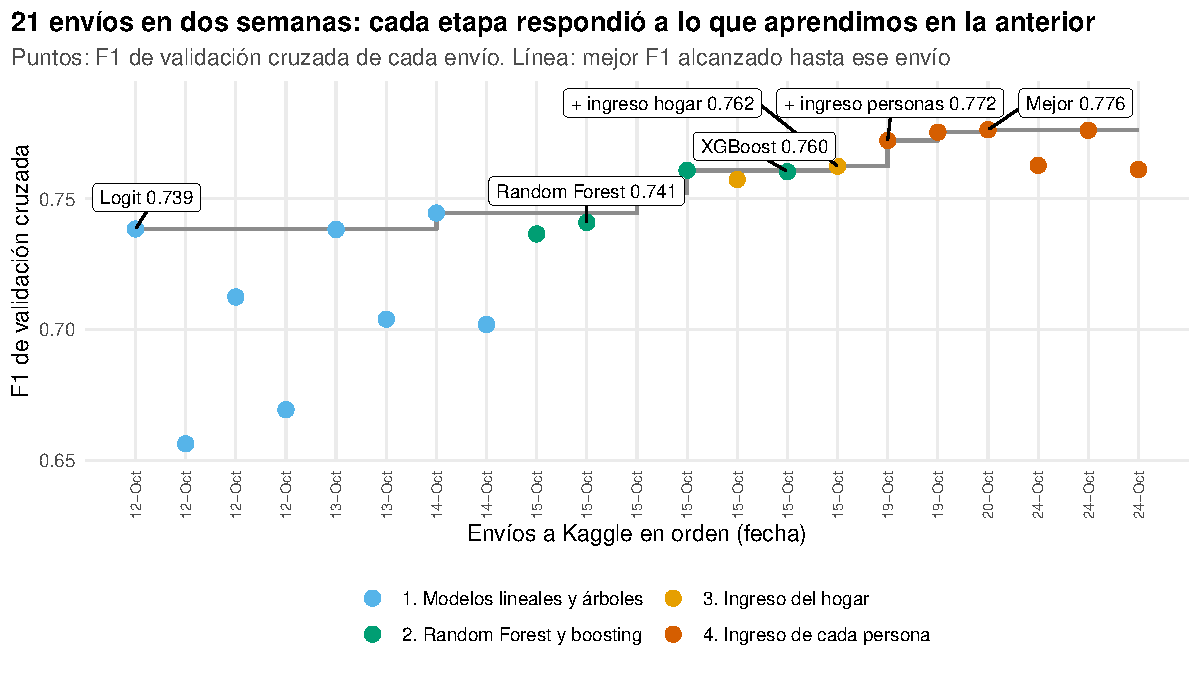
\includegraphics[width=\linewidth]{fig_proceso.pdf}
\end{column}
\begin{column}{0.27\textwidth}
\footnotesize
\textbf{Reglas que mantuvimos en todo el proceso}
\begin{itemize}\setlength\itemsep{0.25em}
\item Los mismos 5 grupos de validación para todos los modelos.
\item Hiperparámetros por búsqueda en grilla con validación cruzada.
\item Umbral: el que maximiza el F1 fuera de muestra.
\item Decidimos con la validación cruzada, no con el puntaje público.
\end{itemize}
\end{column}
\end{columns}
\end{frame}

\begin{frame}{Arquitectura y entrenamiento: del ingreso de cada persona a una probabilidad}
\centering
\resizebox{0.72\linewidth}{!}{% Diagrama del mejor modelo (se usa en los dos decks)
\begin{tikzpicture}[
  font=\scriptsize, >={Stealth[length=2mm]},
  caja/.style={draw=#1, fill=#1!10, rounded corners=3pt, align=center, minimum height=8mm, inner sep=3pt, line width=0.7pt},
  caja/.default=azul, flecha/.style={->, line width=0.7pt, color=gris}]
  % Personas
  \node[caja=naranja, text width=24mm] (per) {\textbf{541 mil personas}\\variables propias\\+ de su hogar};
  \node[caja=naranja, text width=27mm, right=8mm of per, yshift=9mm] (m17) {LightGBM: ingreso total};
  \node[caja=naranja, text width=27mm, right=8mm of per] (m20) {LightGBM: + columnas\\crudas y pesos};
  \node[caja=naranja, text width=27mm, right=8mm of per, yshift=-9mm] (m22) {5 LightGBM: uno por\\componente del ingreso};
  \node[caja=naranja, text width=22mm, right=7mm of m20] (suma) {Suma por hogar\\y promedio: $\hat y$};
  \node[caja=naranja, text width=28mm, right=7mm of suma] (z) {$z = \hat y - g$\\$g$: brecha exacta del DANE\\$\sigma$: error esperado};
  \node[caja=naranja, text width=20mm, below=6mm of z] (logit) {Logit en\\$z,\ z/\sigma,\ \log\sigma$};
  % Hogar
  \node[caja=azul, text width=24mm, below=17mm of per] (hog) {\textbf{165 mil hogares}\\85 variables};
  \node[caja=azul, text width=27mm, right=8mm of hog] (xgb) {XGBoost de\\clasificación};
  % Ensamble
  \node[caja=rosa, text width=34mm, below=6mm of logit] (ens) {$P = 0.3\,P_{\text{XGB}} + 0.7\,P_{\text{ingreso}}$\\pobre si $P \geq 0.40$};
  \draw[flecha] (per.east) -- ++(3mm,0) |- (m17.west);
  \draw[flecha] (per.east) -- (m20.west);
  \draw[flecha] (per.east) -- ++(3mm,0) |- (m22.west);
  \draw[flecha] (m17.east) -- ++(3mm,0) |- (suma.west);
  \draw[flecha] (m20.east) -- (suma.west);
  \draw[flecha] (m22.east) -- ++(3mm,0) |- (suma.west);
  \draw[flecha] (suma) -- (z);
  \draw[flecha] (z) -- (logit);
  \draw[flecha] (logit) -- (ens);
  \draw[flecha] (hog) -- (xgb);
  \draw[flecha] (xgb.east) -- (xgb.east -| ens.west);
\end{tikzpicture}
}
\par\vspace{0.4em}
\tablar{0.86\linewidth}{tab_piezas}
\end{frame}

\begin{frame}{Cada pieza suma: el algoritmo llega a 0.76, la información a 0.78}
\centering
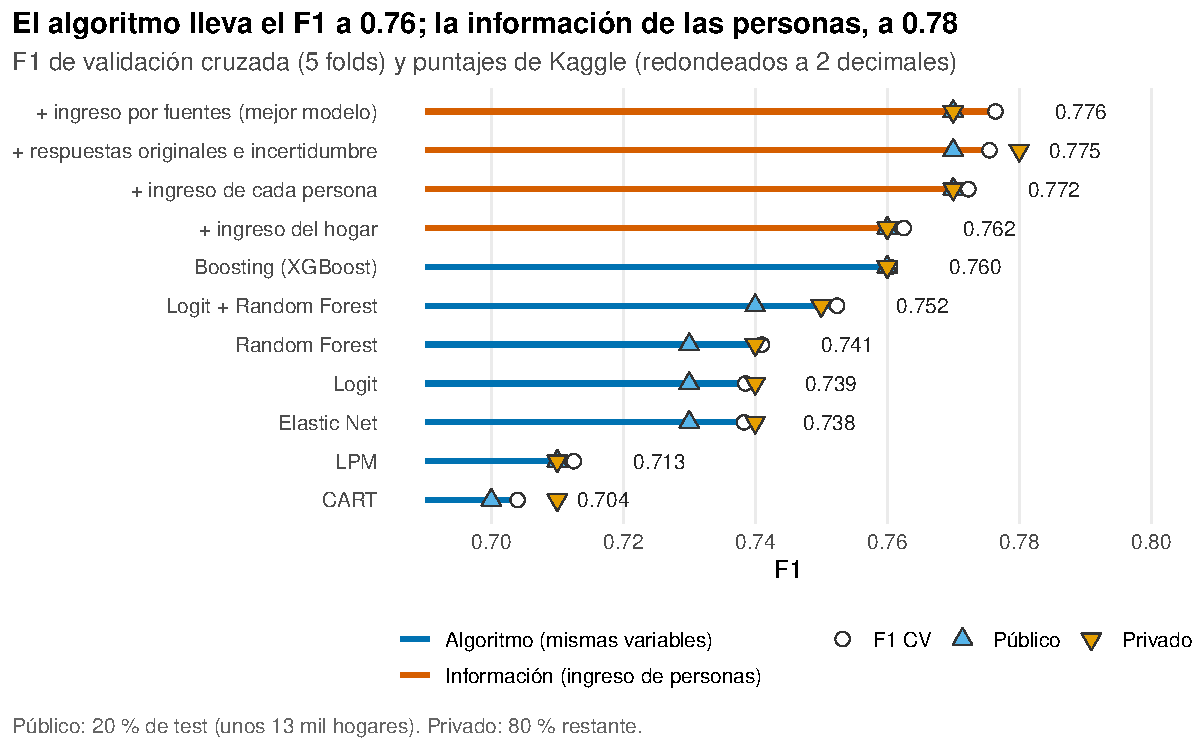
\includegraphics[height=0.86\textheight]{fig_escalera.pdf}
\end{frame}

\begin{frame}{Del ingreso predicho a la probabilidad de ser pobre}
\centering
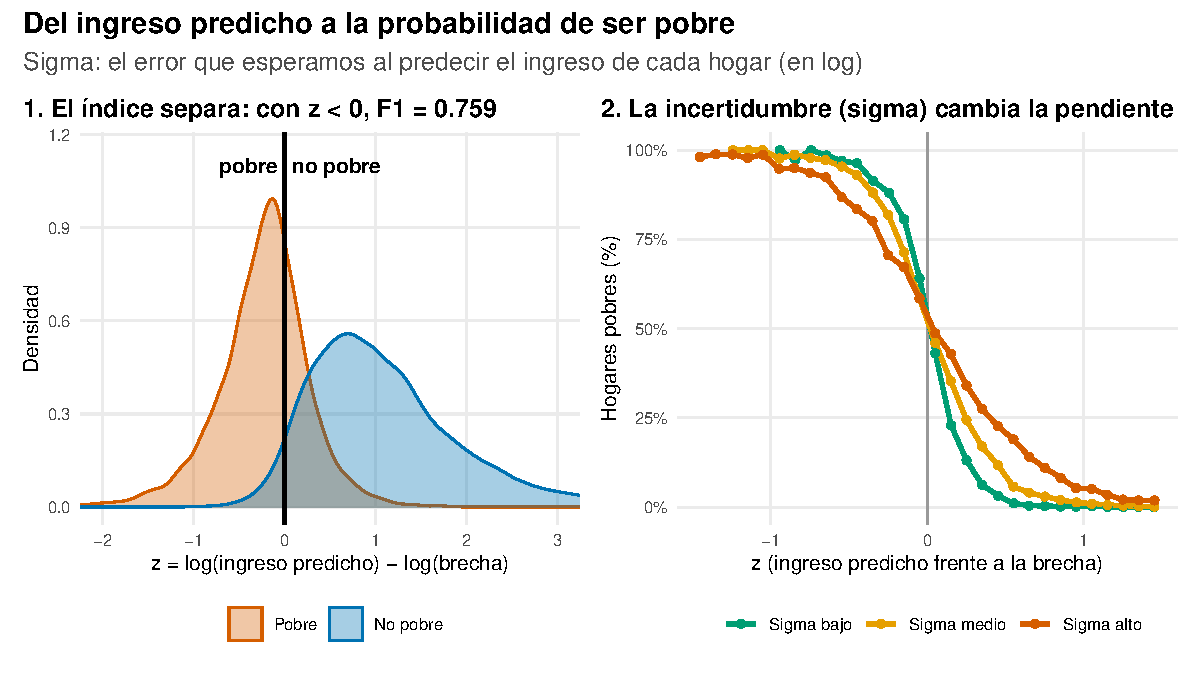
\includegraphics[height=0.73\textheight]{fig_indice_ingreso.pdf}
\par\vspace{0.2em}
{\footnotesize $z$: distancia entre el ingreso predicho y la brecha. $\sigma$: error esperado al predecir el ingreso del hogar.\hspace{1.2em}
$\text{logit}\,P(\text{Pobre}) = b_0 + b_1 z + b_2 \tfrac{z}{\sigma} + b_3 \log\sigma$}
\end{frame}

\begin{frame}{Incertidumbre $\sigma$: la misma distancia a la línea no pesa igual en todos los hogares}
\begin{columns}[c]
\begin{column}{0.56\textwidth}
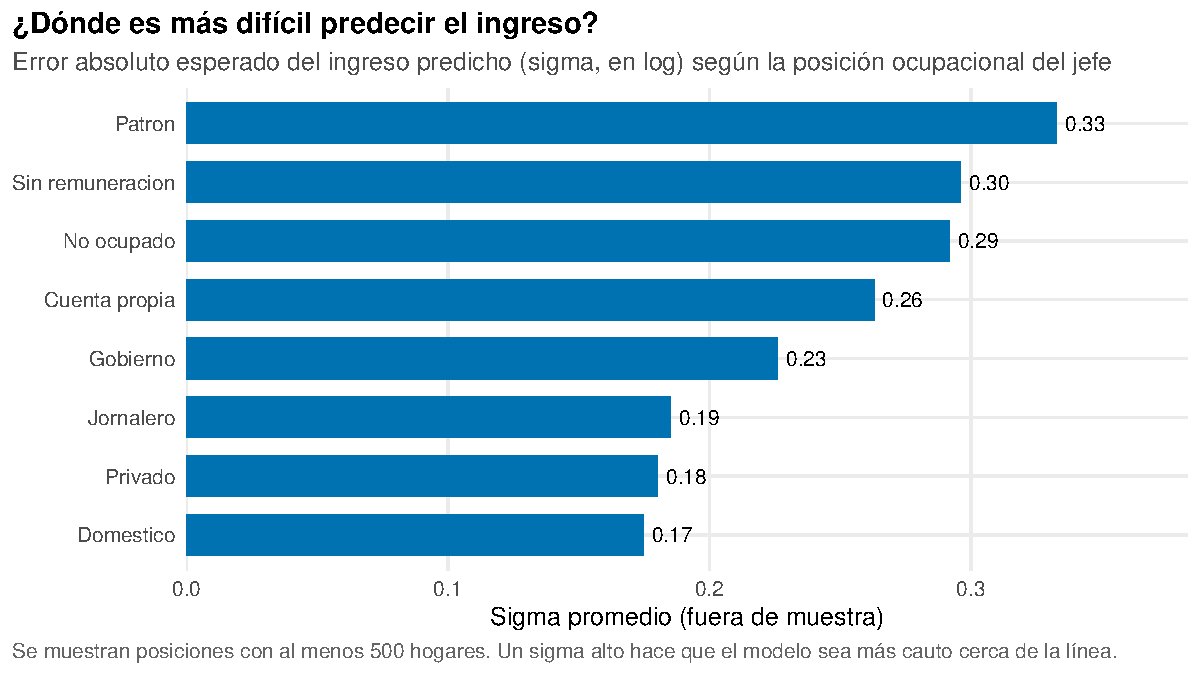
\includegraphics[width=\linewidth]{fig_sigma_posicion.pdf}
\end{column}
\begin{column}{0.42\textwidth}
\begin{block}{Ejemplo: dos hogares con $z = -0.3$}
\small
Ingreso predicho 26 \% por debajo de la brecha. Si el error fuera normal, $P(\text{Pobre}) \approx \Phi(-z/\sigma)$:
\begin{itemize}
\item Jefe asalariado privado, $\sigma = 0.18$: \alert{0.95}
\item Jefe patrón, $\sigma = 0.33$: \alert{0.82}
\end{itemize}
\end{block}
\small
\begin{itemize}\setlength\itemsep{0.25em}
\item Cuenta propia y no ocupados: 64 \% de los hogares y el \alert{83 \%} de los pobres, con $\sigma$ alto.
\item $\sigma$ sube el F1 del ingreso solo de 0.766 a 0.770.
\item Política: verificar en campo los hogares con $\sigma$ alto.
\end{itemize}
\end{column}
\end{columns}
\end{frame}

\begin{frame}{Importancia: vivienda y trabajo formal en el hogar; posición ocupacional en las personas}
\centering
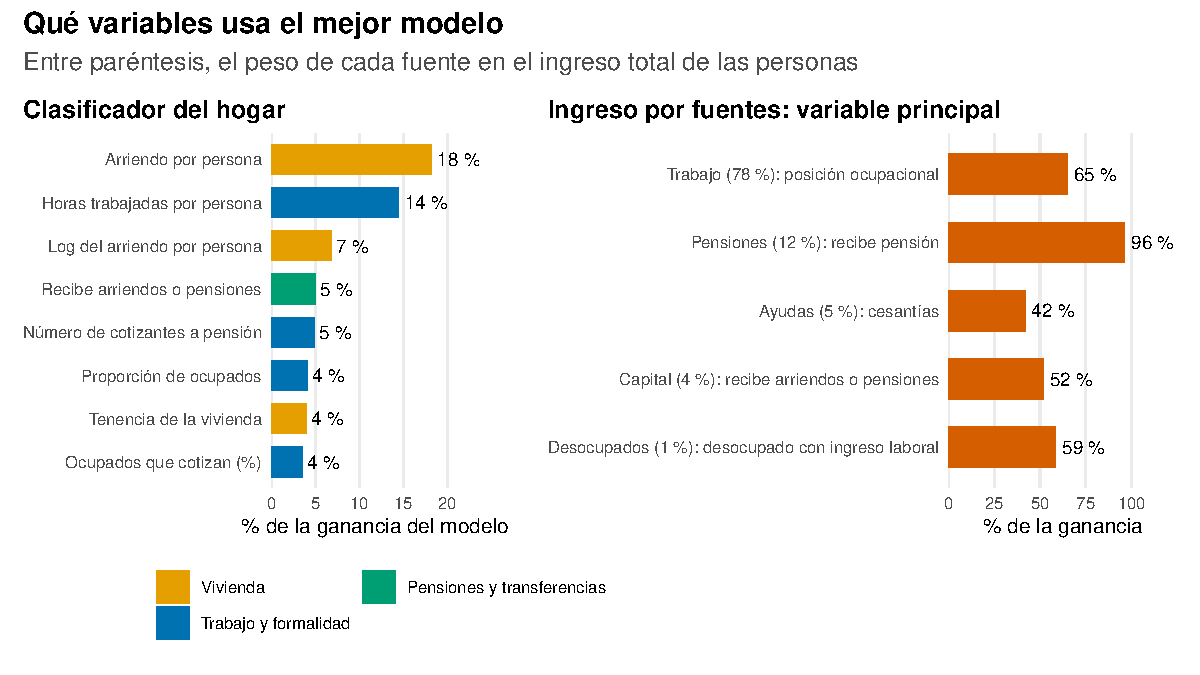
\includegraphics[height=0.86\textheight]{fig_importancia_mejor.pdf}
\end{frame}

\begin{frame}{Diagnóstico: los errores están cerca de la línea}
\begin{columns}[c]
\begin{column}{0.66\textwidth}
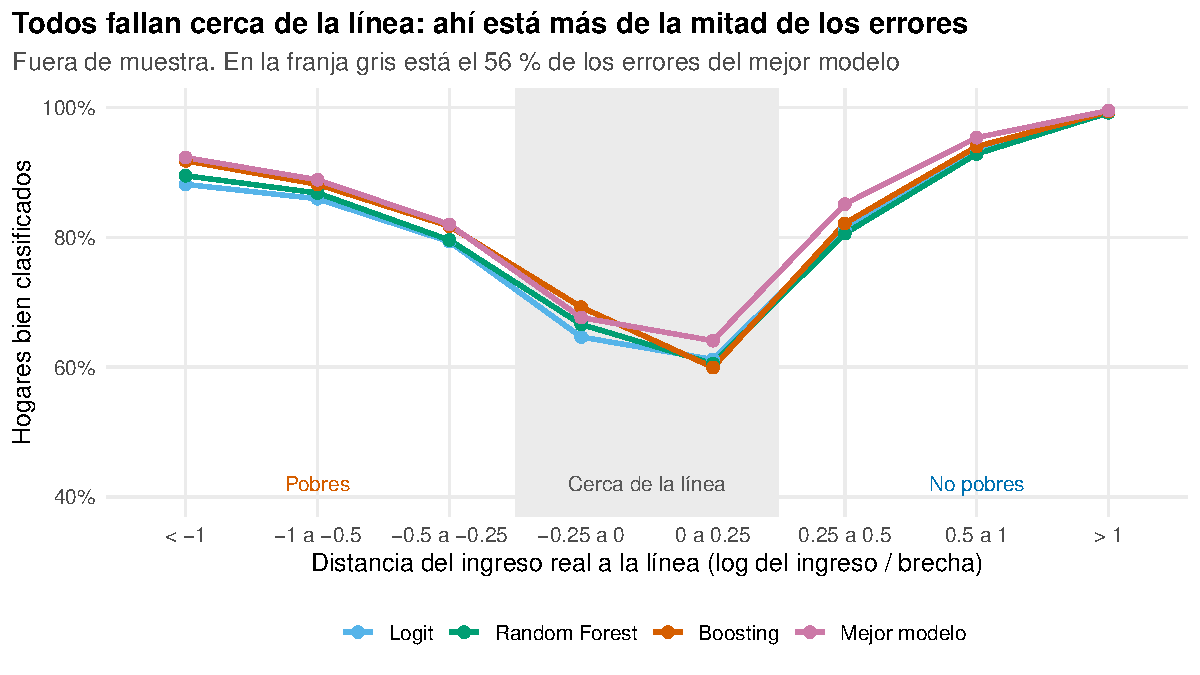
\includegraphics[width=\linewidth]{fig_distancia_linea.pdf}
\end{column}
\begin{column}{0.32\textwidth}
\small
\begin{itemize}\setlength\itemsep{0.3em}
\item El \alert{56 \%} de los errores son hogares a menos de $\pm 0.25$ log de su brecha: ruido casi irreducible.
\item Lejos de la línea acierta más del 90 \%.
\end{itemize}
\vspace{0.3em}
\textbf{F1 por grupo (mejor modelo)}\\[0.3em]
\tablar{0.9\linewidth}{tab_grupos_mejor}
\end{column}
\end{columns}
\end{frame}

\begin{frame}{El desbalance se maneja con el umbral, no rebalanceando}
\begin{columns}[c]
\begin{column}{0.64\textwidth}
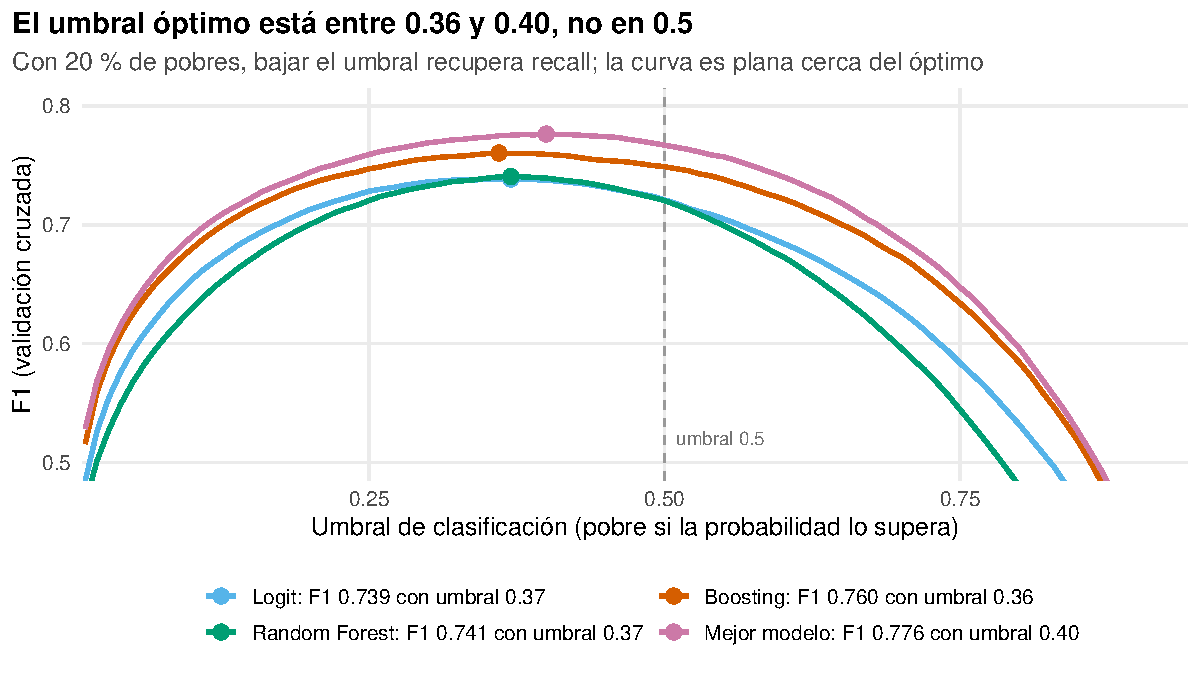
\includegraphics[width=\linewidth]{fig_curvas_umbral.pdf}
\end{column}
\begin{column}{0.34\textwidth}
\small
\begin{itemize}
\item Con umbral 0.5 el mejor modelo pierde 0.01 de F1; el logit, 0.02.
\item \textbf{Rebalancear} (duplicar pobres hasta 50/50) en el árbol: F1 0.702 frente a 0.704. Infla todas las probabilidades, pero el \alert{orden} de los hogares no cambia: el umbral óptimo solo pasó de 0.30 a 0.74.
\item Elegir el umbral por F1 \alert{ya corrige} el desbalance.
\end{itemize}
\end{column}
\end{columns}
\end{frame}

% ------------------------------------------------------------------------------
\section{Implicaciones de política}

\begin{frame}{Matriz de confusión: 1 de cada 5 pobres queda por fuera}
\begin{columns}[c]
\begin{column}{0.58\textwidth}
\centering
\tablar{\linewidth}{tab_confusion}
\par\vspace{1em}
\begin{tabular}{@{}c@{\hspace{2.2em}}c@{\hspace{2.2em}}c@{}}
\cifra{161}{pobres cubiertos} & \cifra{39}{pobres excluidos} & \cifra{54}{no pobres incluidos}\\
\end{tabular}
\par\vspace{0.2em}{\scriptsize Por cada 1,000 hogares, con umbral 0.40 (predicciones fuera de muestra).}
\end{column}
\begin{column}{0.4\textwidth}
\footnotesize
\begin{block}{Dos errores con costos distintos}
\begin{itemize}\setlength\itemsep{0.2em}
\item \textbf{Exclusión} (falso negativo): un pobre queda por fuera; \alert{19.4 \%} de los pobres.
\item \textbf{Inclusión} (falso positivo): un no pobre recibe el beneficio; \alert{25.2 \%} de los beneficiarios.
\end{itemize}
\end{block}
\vspace{0.3em}
\begin{block}{¿Cuánto cuesta cada error?}
Si excluir a un pobre cuesta $c$ veces más que incluir a un no pobre, se marca pobre si $P \geq 1/(1+c)$: con $c = 2$, umbral \alert{0.33}.
\par\vspace{0.2em}
Bajar de 0.40 a 0.30 cuesta solo 0.007 de F1 y sube el recall a 86.5 \%.
\end{block}
\end{column}
\end{columns}
\end{frame}

\begin{frame}{El umbral decide entre errores de exclusión e inclusión}
\begin{columns}[c]
\begin{column}{0.57\textwidth}
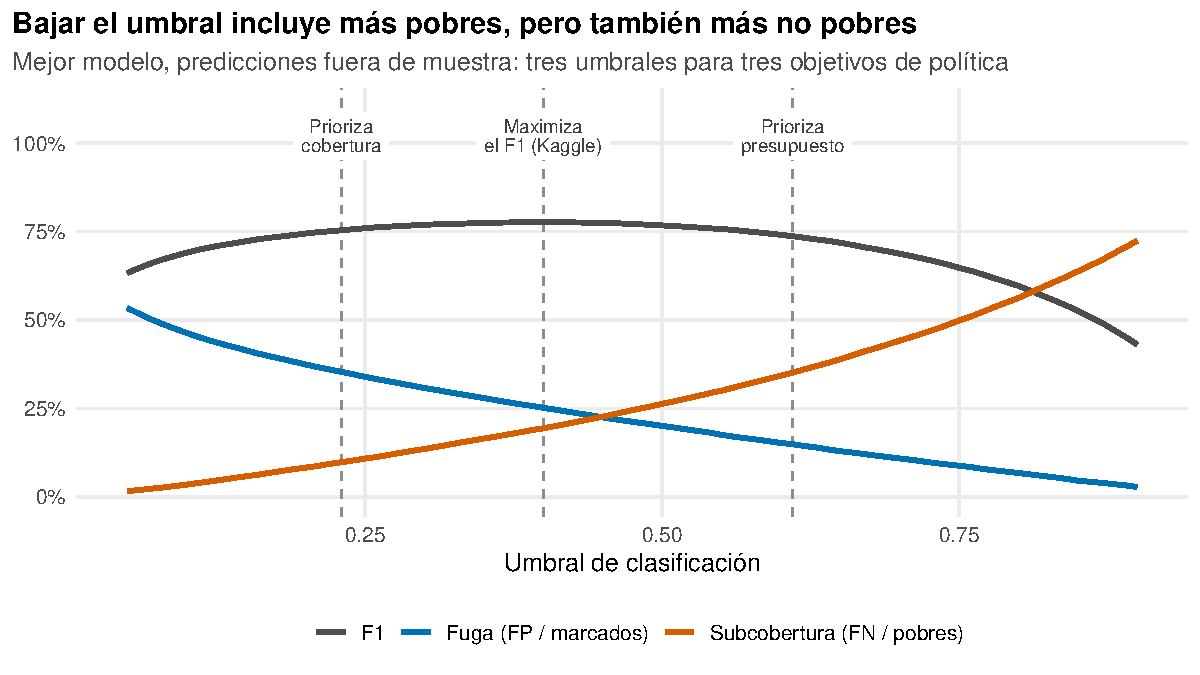
\includegraphics[width=\linewidth]{fig_fuga_subcobertura.pdf}
\par\vspace{0.3em}
\tablar{\linewidth}{tab_escenarios}
\end{column}
\begin{column}{0.38\textwidth}
\footnotesize
\begin{itemize}\setlength\itemsep{0.5em}
\item El F1 pesa igual los dos errores y escoge \alert{0.40}.
\item \textbf{Cobertura} (umbral 0.23): exclusión de 10 \%, inclusión de 35 \%.
\item \textbf{Presupuesto fijo} (0.61): inclusión de 15 \%, exclusión de 35 \%.
\item El umbral se fija según el \alert{costo social} de cada error.
\end{itemize}
\end{column}
\end{columns}
\end{frame}

\begin{frame}{¿Se puede usar con una encuesta corta?}
\begin{columns}[c]
\begin{column}{0.63\textwidth}
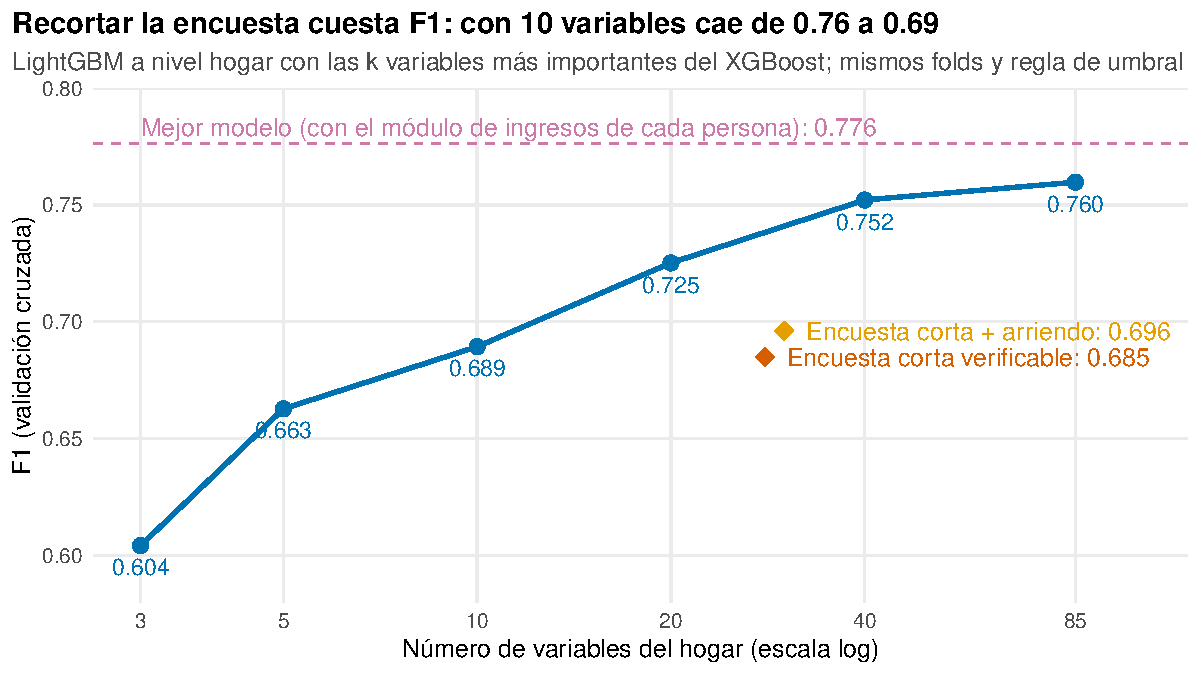
\includegraphics[width=\linewidth]{fig_parsimonia.pdf}
\end{column}
\begin{column}{0.36\textwidth}
\footnotesize
\textbf{Recomendación}
\begin{enumerate}\setlength\itemsep{0.3em}
\item Recortar cuesta: 10 variables dan \alert{0.69}; una encuesta corta \alert{verificable} (vivienda, demografía, ocupados, cotizantes en PILA), 0.685.
\item El módulo de ingresos suma 0.09, pero es caro, y el arriendo autorreportado es \alert{manipulable} con un subsidio en juego.
\item \textbf{Dos etapas:} encuesta corta para todos; módulo completo o visita solo cerca del umbral o con $\sigma$ alto.
\end{enumerate}
\end{column}
\end{columns}
\end{frame}

\begin{frame}{Conclusiones}
\begin{columns}[T]
\begin{column}{0.32\textwidth}
\begin{block}{1. Información}
Entender la regla del DANE y modelar el ingreso de \alert{cada persona} sube el F1 de 0.760 a 0.776. Es la mayor ganancia después de pasar a boosting.
\end{block}
\end{column}
\begin{column}{0.32\textwidth}
\begin{block}{2. Algoritmo y umbral}
Con las mismas variables, el boosting le gana 0.02 al logit y al RF. El \alert{umbral} (0.40) resuelve el desbalance mejor que rebalancear.
\end{block}
\end{column}
\begin{column}{0.32\textwidth}
\begin{block}{3. Política}
El F1 pesa igual los errores de exclusión e inclusión: un programa debe \alert{elegir su umbral}. Una encuesta corta verificable cuesta 0.09 de F1: usarla en dos etapas.
\end{block}
\end{column}
\end{columns}
\vspace{1.2em}
\begin{center}
\cifra{0.776}{F1 validación cruzada}\hspace{2em}\cifra{0.77}{Kaggle público}\hspace{2em}\cifra{0.77}{Kaggle privado}
\end{center}
\end{frame}

\end{document}
